Wiener filtering is commonly used in photography for motion correction/de-blurring. It can also be used for de-noising when the spectral content of the noise is known, even if a system function is not applied.
\section{Definition}
The general assumption of Wiener filtering is that an acquisition is described by
\begin{equation}
 y(t) = (h\circledast x)(t) + n(t)
\end{equation}
where $\circledast$ denotes convolution and:
\begin{itemize}
	\item $ x(t)$ is some original signal (unknown) at time $ t $.
	\item $ h(t)$ is the known impulse response of a linear time-invariant system
	\item $ n(t)$ is some unknown additive noise, independent of $ x(t)$
	\item $ y(t)$ is our observed signal
\end{itemize}
Our goal is to find some $g(t)$ so that we can estimate $x(t)$ as follows:
\begin{equation}\hat {x}(t)=(g\circledast y)(t)\end{equation}
where $\hat {x}(t)$ is an estimate of $x(t)$ that minimizes the mean square error.

The Wiener deconvolution filter provides such a $ g(t)$.  The filter is most easily described in the frequency domain:
\begin{equation}
G(f) = \frac{H^*(f)S(f)}{ |H(f)|^2 S(f) + N(f) }
\end{equation}
where:
\begin{itemize}
\item $ G(f)$ and $ H(f)$ are the Fourier transforms of $ g$ and $ h$, respectively at frequency $ f $.
\item $ S(f)$ is the mean power spectral density of the original signal $ x(t)$
\item $ N(f)$ is the mean power spectral density of the noise $ n(t)$
\item the superscript ${}^*$ denotes complex conjugation.
\end{itemize}
The filtering operation may either be carried out in the time-domain, as above, or in the frequency domain:
\begin{equation}
\hat{X}(f) = G(f)Y(f)
\end{equation}

\section{Example}
The Wiener Filter can be easily implemented in MATLAB, first without noise:
\begin{lstlisting}
I = im2double(imread('cameraman.tif'));
imshow(I);
title('Original Image (courtesy of MIT)');

LEN = 21;
THETA = 11;
PSF = fspecial('motion', LEN, THETA);
blurred = imfilter(I, PSF, 'conv', 'circular');
imshow(blurred);
title('Blurred Image');

wnr1 = deconvwnr(blurred, PSF, 0);
imshow(wnr1);
title('Restored Image');
\end{lstlisting}
See Figure \ref{fig:wiener} to see the result.

\begin{figure}[ht]
	\centering
	\begin{subfigure}[b]{0.3\textwidth}
		\centering
		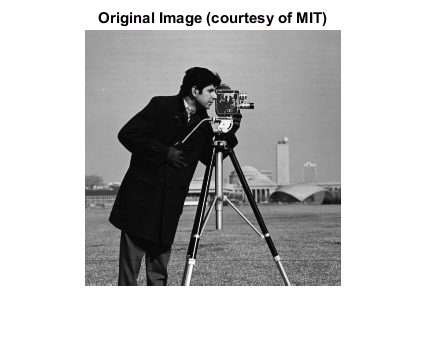
\includegraphics[width=\linewidth]{wiener-original}
		\caption{}
		\label{fig:wiener-original}
	\end{subfigure}\hfill
	\begin{subfigure}[b]{0.3\textwidth}
		\centering
		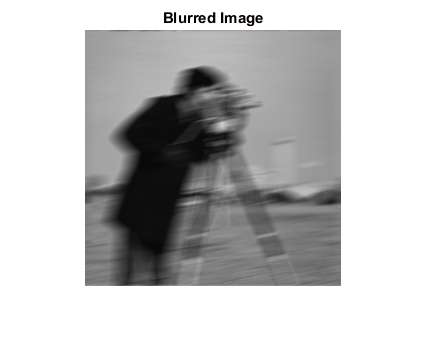
\includegraphics[width=\linewidth]{wiener-blurred}
		\caption{}
		\label{fig:wiener-blurred}
	\end{subfigure}\hfill
	\begin{subfigure}[b]{0.3\textwidth}
		\centering
		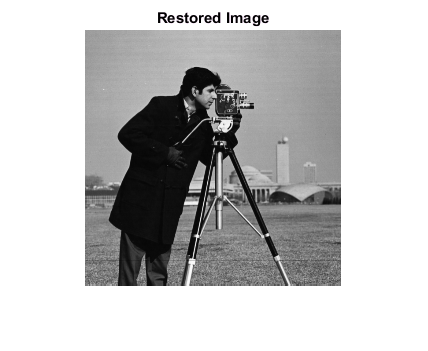
\includegraphics[width=\linewidth]{wiener-restored}
		\caption{}
		\label{fig:wiener-restored}
	\end{subfigure}
	\caption{Wiener Filter Example}\label{fig:wiener}
\end{figure}


The addition of noise makes the deconvolution significantly more temperamental:
\begin{lstlisting}
noise_mean = 0;
noise_var = 0.0001;
blurred_noisy = imnoise(blurred, 'gaussian', ...
noise_mean, noise_var);
imshow(blurred_noisy)
title('Simulate Blur and Noise')

wnr2 = deconvwnr(blurred_noisy, PSF, 0);
imshow(wnr2)
title('Restoration of Blurred, Noisy Image - NSR = 0')

signal_var = var(I(:));
wnr3 = deconvwnr(blurred_noisy, PSF, noise_var / signal_var);
imshow(wnr3)
title('Restoration of Blurred, Noisy Image - Estimated NSR');
\end{lstlisting}

\begin{figure}[ht]
	\centering
	\begin{subfigure}[b]{0.3\textwidth}
		\centering
		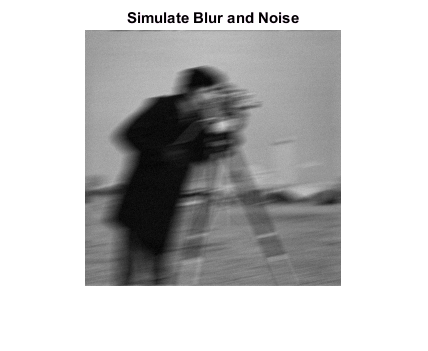
\includegraphics[width=\linewidth]{wiener-noisy}
		\caption{}
		\label{fig:wiener-noisy}
	\end{subfigure}\hfill
	\begin{subfigure}[b]{0.3\textwidth}
		\centering
		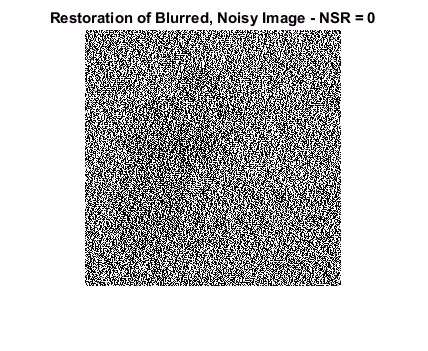
\includegraphics[width=\linewidth]{wiener-noisy-restored}
		\caption{}
		\label{fig:wiener-noisy-restored}
	\end{subfigure}\hfill
	\begin{subfigure}[b]{0.3\textwidth}
		\centering
		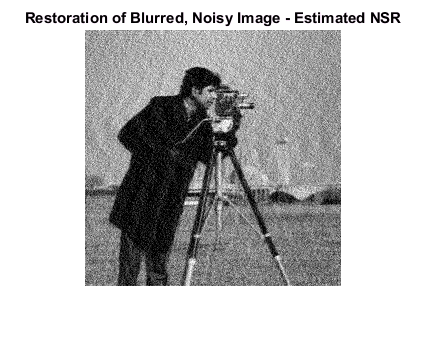
\includegraphics[width=\linewidth]{wiener-noisy-restoredwell}
		\caption{}
		\label{fig:wiener-noisy-restoredwell}
	\end{subfigure}
	\caption{Wiener Filter Example with Noise}\label{fig:wienernoisy}
\end{figure}
